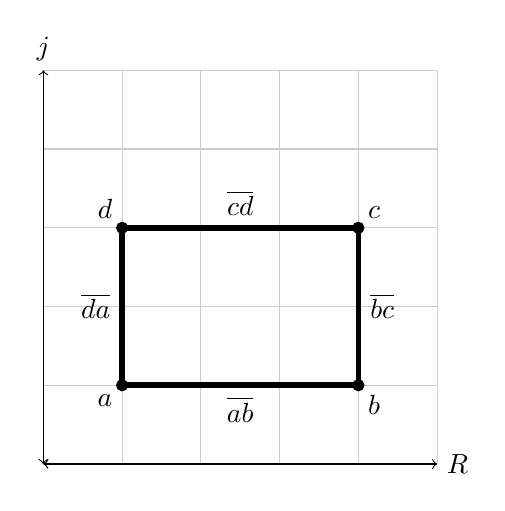
\begin{tikzpicture}
    \draw[thin,gray!40] (0,0) grid (5,5);
    \draw[<->] (0,0)--(5,0) node[right] {$R$};
    \draw[<->] (0,0)--(0,5) node[above]{$j$};
    \coordinate (a) at (1,1);
    \coordinate (b) at (4,1);
    \coordinate (c) at (4,3);
    \coordinate (d) at (1,3);
    
    \draw[fill=black] (a) circle(2pt) node[anchor=north east]{$a$};
    \draw[fill=black] (b) circle(2pt) node[anchor=north west]{$b$};
    \draw[fill=black] (c) circle(2pt) node[anchor=south west]{$c$};
    \draw[fill=black] (d) circle(2pt) node[anchor=south east]{$d$};
    
    \draw[line width=2pt,black,-] (a)--(b) node[midway, below]{$\overline{ab}$};
    \draw[line width=2pt,black,-] (b)--(c) node[midway, right]{$\overline{bc}$};
    \draw[line width=2pt,black,-] (c)--(d) node[midway, above]{$\overline{cd}$};
    \draw[line width=2pt,black,-] (d)--(a) node[midway, left]{$\overline{da}$};
    
\end{tikzpicture}
\caption{Rectángulo en el plano complejo con lineas parametrizadas}